\chapter{Desarrollo y experimentación}
\label{ch:desarrollo}

En este capítulo se describe cómo se construyó el sistema, con qué herramientas y cómo se organizó el código. También se detalla la configuración de los experimentos. El objetivo es facilitar la reproducibilidad del trabajo; para ello, el Anexo~\ref{ch:manual} proporciona instrucciones paso a paso.

\section{El entorno de trabajo}

El desarrollo se realizó en un MacBook Pro con chip M3 Pro y 18\,GB de memoria unificada. A pesar de incluir modelos de deep learning, no fue necesario recurrir a ningún servidor ni GPU externa: TensorFlow es compatible con Apple Silicon y los entrenamientos se completan en pocos minutos. Un portátil moderno resulta suficiente para este tipo de cargas de trabajo.

Se utilizó Python 3.11 con un entorno virtual, lo que evitó numerosos problemas de compatibilidad entre dependencias. En deep learning las versiones resultan determinantes ---un cambio menor en TensorFlow puede dar resultados distintos---, por lo que resulta prácticamente imprescindible fijar las dependencias en un fichero \texttt{requirements.txt}.

\section{Las herramientas}

Python dispone de un ecosistema amplio para análisis de datos. A continuación se enumeran las principales librerías utilizadas:

\begin{itemize}
    \item \textbf{pandas} y \textbf{NumPy}: carga, limpieza y manipulación de datos, junto con operaciones numéricas.
    
    \item \textbf{yfinance}: descarga automatizada del histórico de precios desde Yahoo Finance.
    
    \item \textbf{ta}: cálculo de indicadores técnicos (RSI, MACD, Bandas de Bollinger, etc.).
    
    \item \textbf{scikit-learn}~\cite{pedregosa2011scikit}: implementación de Random Forest y utilidades de preprocesado y evaluación.
    
    \item \textbf{XGBoost}~\cite{chen2016xgboost}: implementación optimizada de \textit{gradient boosting} para árboles.
    
    \item \textbf{statsmodels}: implementación de modelos ARIMA.
    
    \item \textbf{TensorFlow/Keras}~\cite{abadi2016tensorflow}: implementación de los modelos de aprendizaje profundo.
    
    \item \textbf{matplotlib} y \textbf{seaborn}: generación de figuras para el análisis y su inclusión en LaTeX.
\end{itemize}

\section{Organización del código}

Se mantuvo una estructura modular ---lo que inicialmente puede parecer excesivo resulta ventajoso cuando es necesario modificar o ampliar el sistema---. El directorio principal tiene subdirectorios para datos crudos y procesados, código fuente, scripts, resultados y documentación. Dentro del código, descarga, preprocesado, modelos y evaluación viven en módulos separados.

\begin{verbatim}
tfg/
+-- data/
|   +-- raw/          # Datos tal como se descargan
|   +-- processed/    # Datos listos para modelar
+-- src/
|   +-- data/         # Descarga y preprocesado
|   +-- models/       # Implementacion de modelos
|   +-- evaluation/   # Validacion y metricas
|   +-- utils/        # Reproducibilidad y utilidades
+-- scripts/          # Scripts de ejecucion
+-- results/          # Resultados (CSV) y plots
|   +-- plots/        # Figuras generadas
+-- memoria/          # Este documento
|   +-- Imagenes/     # Figuras incluidas en LaTeX
+-- main.py           # Punto de entrada principal
+-- requirements.txt  # Dependencias del proyecto
\end{verbatim}

Cada módulo tiene una responsabilidad delimitada: el descargador se encarga exclusivamente de la adquisición de datos y el preprocesador, de su transformación. Esta separación facilita las pruebas y el mantenimiento. La incorporación de un nuevo modelo se realiza añadiendo su implementación en \texttt{src/models/} y conectándolo desde los scripts de ejecución, sin reestructurar el resto del proyecto.

Los scripts de ejecución están en la carpeta \texttt{scripts/}. El orquestador principal es \texttt{run\_all\_\allowbreak experiments.\allowbreak py}, que genera los resultados de los experimentos A--D. Posteriormente se ejecuta \texttt{run\_additional\_\allowbreak metrics.\allowbreak py} para las métricas direccionales y el test de Diebold-Mariano, \texttt{generate\_all\_\allowbreak plots.\allowbreak py} y \texttt{generate\_\allowbreak summary\_\allowbreak plots.\allowbreak py} para las figuras, y \texttt{export\_\allowbreak tables\_\allowbreak to\_\allowbreak latex.\allowbreak py} para las tablas. Para ejecutar todo de principio a fin, se utiliza \texttt{main.py}. Los fragmentos de código más relevantes se pueden consultar en el Anexo~\ref{ch:codigo}.

\section{Flujo de trabajo del sistema}

Esta sección describe las cuatro etapas principales del pipeline: la descarga de datos desde las fuentes externas, el preprocesamiento y cálculo de indicadores, el entrenamiento y predicción con los modelos, y finalmente la evaluación de resultados. La Figura~\ref{fig:pipeline} muestra el flujo de trabajo completo del sistema.

\begin{figure}[H]
\centering
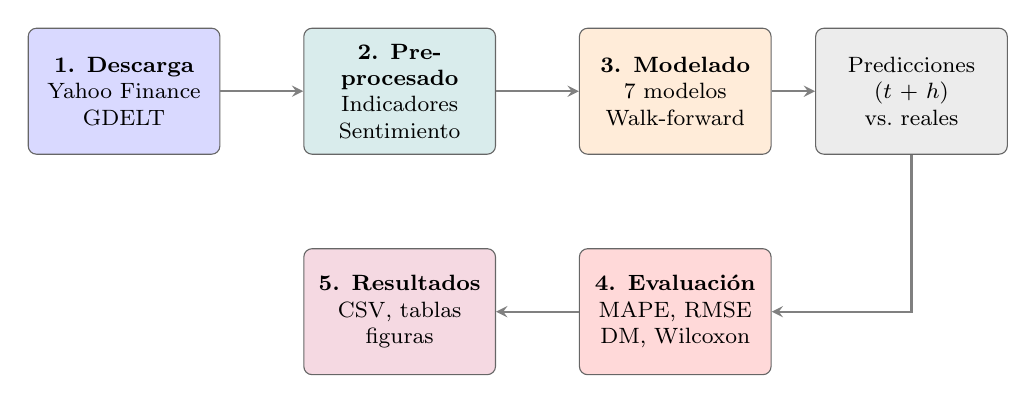
\begin{tikzpicture}[
  block/.style={rectangle, rounded corners=3pt, draw=black!60, fill=#1!15,
    minimum width=2.4cm, minimum height=1.6cm, text centered, text width=2.2cm,
    font=\footnotesize},
  arr/.style={->, >=stealth, thick, draw=black!50},
  lbl/.style={font=\scriptsize\itshape, text=black!50}
]
  % Fila superior
  \node[block=blue]   (dl)  at (0,0)    {\textbf{1. Descarga}\\Yahoo Finance\\GDELT};
  \node[block=teal]   (pp)  at (3.5,0)  {\textbf{2. Preprocesado}\\Indicadores\\Sentimiento};
  \node[block=orange] (mod) at (7,0)    {\textbf{3. Modelado}\\7 modelos\\Walk-forward};
  % Fila inferior
  \node[block=red]    (eva) at (7,-2.8) {\textbf{4. Evaluación}\\MAPE, RMSE\\DM, Wilcoxon};
  \node[block=purple] (res) at (3.5,-2.8){\textbf{5. Resultados}\\CSV, tablas\\figuras};
  % Predicciones
  \node[block=gray]   (pred) at (10,0)  {Predicciones\\$(t+h)$\\vs.\ reales};
  % Flechas
  \draw[arr] (dl)  -- (pp);
  \draw[arr] (pp)  -- (mod);
  \draw[arr] (mod) -- (pred);
  \draw[arr] (pred) |- (eva);
  \draw[arr] (eva) -- (res);
\end{tikzpicture}
\caption{Flujo de trabajo del sistema de predicción.}
\label{fig:pipeline}
\end{figure}

El proceso completo tiene cuatro etapas:

\subsection{Descarga de datos}

El módulo de descarga se conecta a Yahoo Finance y a la API de GDELT. Para cada activo, guarda un CSV con el histórico de precios. Para el sentimiento, guarda otro CSV con el índice específico del activo.

La implementación se mantiene deliberadamente sencilla: para los precios se utiliza \texttt{yf.download} con el ticker y el rango de fechas; para el sentimiento se realizan peticiones HTTP a GDELT y se construye un índice diario a partir de la serie devuelta por la API.

Se ha añadido manejo de errores y reintentos: si una descarga falla, el proceso se detiene para no propagar datos incompletos. En un sistema de producción se requeriría mayor robustez; no obstante, el nivel alcanzado resulta adecuado para un proyecto académico.

\subsection{Preprocesado}

El preprocesador carga los CSVs crudos y los transforma. Los pasos principales son:

1. Cargar los precios y detectar el formato del fichero (yfinance tiene una cabecera multinivel no estándar).

2. Calcular los indicadores técnicos: SMA de 20 y 50 días, RSI con periodo 14, MACD y su señal, Bandas de Bollinger (banda alta y baja).

3. Cargar el fichero de sentimiento, normalizar columnas a \texttt{Sentiment\_Index} y \texttt{Sentiment\_Volume} (cuando existe), y fusionarlo con los precios por fecha. Los días sin valor de sentimiento se rellenan con el último conocido (forward fill), siempre usando el valor pasado más reciente y sin mirar al futuro.

4. Crear las variables objetivo. Para cada horizonte (1, 3, 7, 14 y 30 días), se calcula el rendimiento logarítmico futuro y su dirección; el precio futuro se reconstruye después en la evaluación.

5. Eliminar las filas con valores nulos (las primeras por falta de historia para los indicadores, las últimas porque no tienen futuro).

6. Guardar el resultado en \texttt{data/processed/}.

Todo esto está encapsulado en una clase \texttt{DataPreprocessor} que se puede reutilizar para cada activo.

\subsection{Entrenamiento y predicción}

Los scripts de modelos cargan los datos preprocesados y ejecutan el entrenamiento con validación walk-forward.

Para los modelos de ML clásico, es necesario crear previamente las características. Se utilizan retardos del precio y de los indicadores: el valor de hace 1, 2, 3... días. Con esto se convierte el problema de series temporales en uno de regresión tabular estándar.

En la práctica, se utilizan retardos de 10 días para \texttt{Close}, \texttt{RSI}, \texttt{MACD} y las variables de sentimiento (\texttt{Sentiment\_Index} y \texttt{Sentiment\_Volume}). El objetivo es el log-retorno a $h$ días, y el precio se reconstruye multiplicando por el cierre de referencia. Para evitar fuga en validación walk-forward, en cada fold se recortan las últimas $h$ observaciones del bloque de entrenamiento, ya que su objetivo dependería de precios del bloque de test.

Para los modelos de deep learning, la preparación es diferente. Se escalan las características de entrada al rango [0,1] con MinMaxScaler (ajustado solo en los datos de entrenamiento para evitar fuga de información). En este punto se excluyen explícitamente las columnas \texttt{Target\_*}, ya que están calculadas con \texttt{shift(-h)} y contienen información futura. Luego se crean secuencias tridimensionales: cada muestra es una ventana de 30 días con todas las características.

El entrenamiento sigue el flujo habitual. Para Random Forest y XGBoost se ajusta el modelo con \texttt{fit} y se generan predicciones con \texttt{predict}. En redes neuronales se define la arquitectura con Keras, se compila con Adam y pérdida MSE, y se entrena durante 10 épocas.

\subsection{Evaluación}

Después de cada iteración de walk-forward, se calculan RMSE, MAE y MAPE comparando predicciones con valores reales~\cite{hyndman2006another}. Además, se calculan métricas direccionales (DA, F1, MCC) para capturar si el modelo acierta la subida o bajada. Finalmente, las métricas se promedian a lo largo de todas las iteraciones para obtener una estimación más estable.

Para la ablación con/sin sentimiento se aplica un test de Wilcoxon pareado sobre las métricas por fold, de modo que la comparación no sea solo descriptiva sino también estadística.

Los resultados se guardan en CSVs: uno por experimento, con columnas para el activo, el modelo, la iteración y las métricas. Esto facilita el análisis posterior y la generación de gráficas.

Además se añadió un script para exportar las tablas de resultados directamente a LaTeX (\texttt{scripts/export\_tables\_to\_latex.py}). Así, tras volver a ejecutar los experimentos, las tablas de la memoria se actualizan de forma automática.

\section{Los modelos en detalle}

\subsection{El predictor naive}

El predictor naive se define de la forma más simple posible: el precio predicho para dentro de $h$ días es el precio actual ($t$). A pesar de su simplicidad, puede ser difícil de batir en mercados cercanos a la eficiencia.

\subsection{ARIMA}

Se utilizó la implementación de statsmodels. El modelo ARIMA$(5,1,0)$ tiene cinco coeficientes autorregresivos y una diferenciación~\cite{box2015time}. La diferenciación convierte la serie de precios en rendimientos, que son más estacionarios.

El ajuste es automático: statsmodels estima los parámetros por máxima verosimilitud. Para mantener la comparabilidad con el resto de modelos, ARIMA se ajusta una vez por fold y, durante el bloque de test, solo se actualiza el estado con la observación más reciente (\textit{append} sin \textit{refit}) antes de generar la predicción a $h$ pasos. De ese modo no se reestiman parámetros en cada fecha de test.

\subsection{Random Forest}

Se configuraron 100 árboles~\cite{breiman2001random} y se fijó la semilla para reproducibilidad. El resto de hiperparámetros queda en valores por defecto, lo que da un baseline razonable sin tuning.

Las características de entrada son los retardos de 10 días de \texttt{Close}, \texttt{RSI}, \texttt{MACD}, \texttt{Sentiment\_Index} y \texttt{Sentiment\_Volume}. Esto da un vector de 50 dimensiones cuando todas las columnas están presentes, suficiente para capturar dinámica reciente sin inflar demasiado la complejidad.

\subsection{XGBoost}

Similar configuración: 100 rondas de boosting y tasa de aprendizaje de 0.1. El resto de parámetros se dejan por defecto para tener un punto de partida estable.

XGBoost tiende a funcionar mejor que Random Forest cuando hay interacciones complejas entre variables, aunque es más sensible a la elección de hiperparámetros. Usa exactamente el mismo conjunto de características que el Random Forest.

\subsection{LSTM y GRU}

La arquitectura de ambas es muy similar~\cite{hochreiter1997long, cho2014learning}:

\begin{verbatim}
Capa recurrente (50 unidades, return_sequences=True)
Dropout (20%)
Capa recurrente (50 unidades)
Dropout (20%)
Capa densa (25 neuronas)
Capa de salida (1 neurona)
\end{verbatim}

La diferencia es el tipo de celda: LSTM tiene tres puertas, GRU tiene dos. En la práctica, GRU entrena más rápido y a menudo da resultados comparables.

El entrenamiento se realiza con Adam (tasa de aprendizaje por defecto de 0.001) y pérdida MSE. Con 10 épocas suele ser suficiente; a partir de ahí aumenta el riesgo de sobreajuste.

\subsection{CNN 1D}

La arquitectura es más sencilla:

\begin{verbatim}
Conv1D (64 filtros, kernel=2, ReLU)
Flatten
Capa densa (50 neuronas, ReLU)
Capa de salida (1 neurona)
\end{verbatim}

Las convoluciones capturan patrones locales de 2 días consecutivos y luego aplanan la salida para pasarla a la parte densa. Es más rápida de entrenar que las recurrentes.

\section{Configuración de los experimentos}

\subsection{Periodo de datos}

Los datos se descargan desde noviembre de 2020 hasta noviembre de 2025. Tras el período de calentamiento de indicadores técnicos y alineación con sentimiento, el dataset efectivo empieza en enero de 2021. El intervalo cubre regímenes distintos: el rally alcista de 2021, la corrección severa de 2022 y el periodo de recuperación posterior. Esta diversidad resulta relevante para evaluar la robustez de los modelos ante cambios de régimen.

\subsection{Horizontes de predicción}

En los experimentos reportados se analizaron tres horizontes: 1 día (muy corto plazo), 7 días (horizonte principal) y 30 días (medio plazo). En general, se espera que el error aumente con el horizonte, ya que la incertidumbre se acumula y la probabilidad de eventos inesperados es mayor en ventanas más largas. Aunque en preprocesado también se generan objetivos a 3 y 14 días para facilitar extensiones del pipeline, esos dos horizontes no forman parte de los resultados A--D presentados en esta memoria.

\subsection{Validación walk-forward}

Se realizaron 12 iteraciones de walk-forward~\cite{hyndman2021forecasting}. En cada iteración, se entrena con todos los datos anteriores a un punto de corte y se evalúa sobre los 30 días siguientes. Los puntos de corte están distribuidos uniformemente a lo largo del dataset.

Doce iteraciones proporcionan un test total de 360 días. Se trata de una muestra más amplia que reduce la varianza de los resultados, aunque sigue siendo limitada frente a todo el histórico.

Dentro de cada bloque de 30 días se generan 30 predicciones a horizonte fijo ($t+h$), una por día, utilizando únicamente datos observados hasta ese día. No se emplea predicción recursiva ni sustitución de valores reales por predicciones.

\subsection{Hiperparámetros}

No se realizó una búsqueda exhaustiva de hiperparámetros. Se utilizaron valores por defecto razonables basados en la literatura. Se trata de una decisión deliberada: el objetivo era comparar familias de modelos, no optimizar al máximo cada uno.

Es importante reconocer que con tuning cuidadoso los resultados podrían mejorar, especialmente para los modelos de deep learning. Esta es una limitación del trabajo.

\subsection{Semillas y reproducibilidad}

Para poder repetir los resultados, se fijó una semilla global (42) en Python, NumPy y TensorFlow, y se activaron operaciones deterministas cuando es posible. Además, la semilla se reinicia al inicio de cada entrenamiento (por fold y modelo) para que las comparativas sean consistentes. En CPU los resultados son idénticos entre ejecuciones; en GPU puede haber ligeras variaciones por la propia naturaleza del hardware.

\section{Los cuatro experimentos}

Para estructurar el análisis, se diseñaron cuatro experimentos:

\textbf{Experimento A: Comparación de modelos.} Todos los modelos, todos los activos, horizonte de 7 días. Se utiliza el conjunto completo de variables (incluyendo sentimiento cuando aplica) para tener un ranking general de rendimiento.

\textbf{Experimento B: Impacto del horizonte.} Los modelos de deep learning sobre Bitcoin con horizontes de 1, 7 y 30 días. El objetivo es analizar cómo degrada la predicción a mayor plazo.

\textbf{Experimento C: Ablación del sentimiento.} Modelos DL con y sin la variable de sentimiento, todos los activos. Este es el experimento central para responder a la pregunta de investigación.

\textbf{Experimento D: Periodos de mercado.} Se utilizan los tres modelos de aprendizaje profundo (LSTM, GRU y CNN) en Bitcoin para tres periodos distintos: bull market 2021, bear market 2022, y periodo reciente. En cada periodo se hace una partición 80/20 (train/test) y se evalúa con horizonte 7. El objetivo es ver si los modelos se comportan de forma similar o divergente ante distintos regímenes de mercado.

\section{Generación de visualizaciones}

Para presentar los resultados de forma clara y facilitar su interpretación, se generaron aproximadamente cuarenta gráficas que cubren diferentes aspectos de los experimentos. El diseño de cada tipo de visualización responde a un objetivo específico:

\begin{itemize}
    \item \textbf{Gráficas de barras por modelo y activo:} Permiten comparar el MAPE de cada modelo de forma inmediata. Son útiles para identificar qué modelo funciona mejor en cada activo y detectar patrones generales (por ejemplo, que los baselines Naive/ARIMA se mantienen como referencia difícil de batir y que los modelos DL quedan por detrás en esta configuración experimental).
    
    \item \textbf{Gráficas de evolución por horizonte:} Muestran cómo evoluciona el error a medida que aumenta el horizonte de predicción. Estas líneas ayudan a entender el trade-off entre plazo y precisión, y a identificar qué modelos degradan más rápidamente.
    
    \item \textbf{Mapas de calor (heatmaps):} Resumen el impacto del sentimiento por modelo y activo en una matriz compacta. Los colores facilitan la identificación de patrones: verde indica mejora al incluir sentimiento, rojo indica perjuicio.
    
    \item \textbf{Gráficas de predicción vs. realidad:} Superponen la serie de precios reales con las predicciones del modelo para casos concretos. Proporcionan una intuición visual de cómo de cerca siguen las predicciones a la realidad y permiten detectar sesgos sistemáticos (por ejemplo, si el modelo suaviza demasiado o reacciona tarde a cambios bruscos).
    
    \item \textbf{Diagramas de caja (boxplots):} Muestran la distribución del error por modelo, incluyendo mediana, cuartiles y valores atípicos. Son esenciales para evaluar la consistencia: un modelo con baja media pero alta dispersión puede ser menos fiable que otro con error medio algo mayor pero más estable.
\end{itemize}

Todo el proceso de generación está automatizado mediante scripts de Python ubicados en \texttt{scripts/}. El script principal \texttt{generate\_all\_plots.py} produce las gráficas experimentales, mientras que \texttt{generate\_summary\_plots.py} crea las visualizaciones de síntesis. Las imágenes se guardan en \texttt{results/plots/} y posteriormente se copian a \texttt{memoria/Imagenes/} para su inclusión en el documento LaTeX. Esta separación permite regenerar las visualizaciones sin afectar al resto de archivos del proyecto.
